\section{Исследование и построение решения задачи}
\label{sec:Chapter3} \index{Chapter3}
С целью исследования и разработки своих собственных OSINT методов сбора информации о человеке с помощью поисковых сервисов и 
социальных сетей предстоит решить следующие задачи:
\begin{itemize}
    \item поисковые сервисы:
    \begin{enumerate}
        \item Определить структуру поискового сайта. В качестве таких сайтов возьмем следующие ресурсы:
        \begin{itemize}
            \item DuckDuckGo;
            \item Google;
            \item Yandex;
            \item Yahoo.
        \end{itemize}
        \item Извлечение найденных ссылок по заданному ключевому слову.
        \item Сбор информации с сайтов по отобранным ссылкам.
        \item Для случая с Google попробовать Google Search API: определить шаблон GET-запроса, структуру возвращаемых данных.
    \end{enumerate}
    \item социальные сети:
    \begin{enumerate}
        \item Определить структуру сайта социальной сети. Будем работать над социальной сетью LinkedIn.
        \item Реализовать поиск и сбор данных пользователей и организаций посредством веб-краулинга сайта.
        \item Реализовать сбор данных пользователей и организаций посредством закрытого API LinkedIn. Для этого потребуется:
        \begin{itemize}
            \item реализовать вход систему через закрытое API посредством GET и POST запросов;
            \item определить шаблон GET-запроса для получения данных по указанным ключевым словам, структуру возвращаемых данных.
        \end{itemize}
    \end{enumerate}
    \item реализовать все указанные выше подзадачи в систему сбора данных. 
\end{itemize}

\subsection{Исследование архитектуры сборщиков Scrapy}

Поскольку основным фреймворком для сбора данных является Scrapy, то необходимо изначально ознакомиться с его архитектурой.
\cite{scrapyArchitecture}

\begin{figure}[H]
    \center{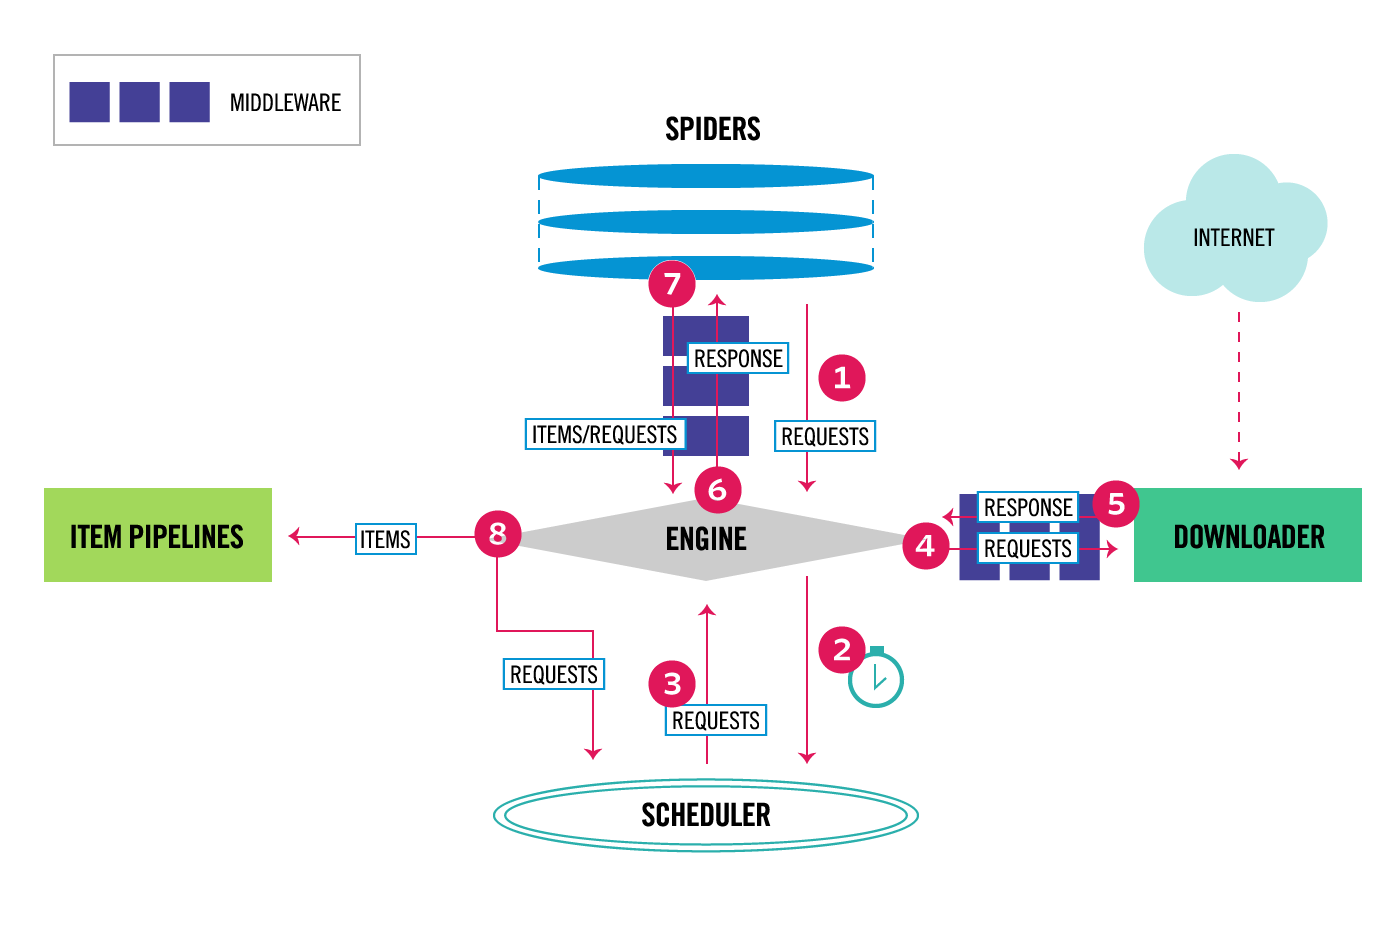
\includegraphics[height=6cm,keepaspectratio]{pictures/scrapy_architecture.png}}
    \caption{Архитектура Scrapy spider.}
    \label{ris:image}
\end{figure}

\par
Из рисунка видно, что изначально из spider'ов запросы направляются в движок и планировщик, затем через промежуточный загрузчик
запросы выполяются в сети Интернет. Ответ от ресурсов возвращается в загрузчик, оттуда обратно в движок и в конвейер элементов.
В нашей задаче потребуется писать собственные downloader middlewares и pipelines, помимо самих spiders непосредственно.

\subsubsection{Scrapy Downloader Middleware} 
Обусловленно это тем, что на этапе, когда запрос находится в загрузчике, есть возможность загрузить api-токен, логин и пароль,
или cookie-файлы для браузера и подставить его в запрос (переопределяемый метод process\_request). 
В случае, если учетных данных нет, то в загрузчике можно составить несколько вспомогательных запросов, которые нагенерируют 
новые cookie-файлы и подставят в исходный запрос. Также есть возможность обработать ответ в методе process\_response. 
Этот метод может использоваться для обновления учетных данных, кодов ответа, отличных от 200, но которые допустимы для запроса.
Стоит отметить, что каждый запрос, запущенный внутри проекта, будет проходить через process\_request и process\_response. Это
образует некую рекурсию и сложности для понимания, от какого именно запроса мы получили ответ.  

\subsubsection{Scrapy Item Pipelines}  
Изначально Scrapy просто собирает данные в некий массив структур, который можно выгрузить в json файл. Но фреймворк также 
поддерживает функционал скачивания файлов по их url. Для изображений используется встроенный ImagePipeline, для файлов --
FilesPipeline. Но есть потребность иногда рендерить веб-страницы полностью, так как Scrapy не поддерживает выполнение JavaScript
файлов. Для рендера html страниц будем использовать Splash\footnote{https://splash.readthedocs.io/en/stable/} и фреймворк 
scrapy-splash\footnote{https://github.com/scrapy-plugins/scrapy-splash}. Таким образом, для выгрузки наибольшего количества
данных, документов и изображений с веб-страниц будет использовать SplashRequest, который вернет текст html-страницы с всеми
отработанными JavaScript-скриптами.

\subsection{Извлечение информации из страниц}
В то время как Scrapy используется для навигации и перехода по ссылкам, отправке запросов и получения ответов от сайтов, в то же
время он не может самостоятельно структурировать полученную информацию. Инструменты для извлечения данных с веб-страницы следующие:
CSS-селекторы, Xpath-селекторы \cite{cssXpathSelectors}. С помощью них можно извлекать данные из объекта Response, который 
предоставляет Scrapy после выполнения запроса. Это стандартные технологии для извлечения данных с html страниц, они весьма
универсальны, но имеют один перечень минусов:
\begin{itemize}
    \item для того, чтоб их задействовать необходимо загрузить html страницу, зачастую
    содержащую лишние данные, перед применением надо ждать выполнения всех скриптов на сайте;
    \item сайты очень часто меняют свою верстку в следствие чего селекторы могут стать неактуальным (перестать работать 
    или собирать некорректные данные);
    \item многие популярные сайты имеют защиту, шифрование против извлечения данных при помощи селекторов, которые искажают
    ключевые поля (имена классов, id атрибутов), что усложняет со временем составление и поддержку программы.
\end{itemize} 

\subsection{Поиск информации в поисковом портале при помоще Google API Search}
Поскольку поиск и извлечение информации с помощью CSS-селекторов весьма дорогостоящее по времени занятие, было решено 
исследовать другие способы поиска данных в Google. Инструментом, который решал бы вопросы затрат времени стал Google API Search.
Он обрабатывает ровно те же запросы и возвращает JSON-файл с результатами поиска. И поиск посредством api куда более производительное
и стабильное, то есть теперь не нужно привязывать на CSS-селекторы, которые могут стать невалидными в любое время. А поскольку
данное API является открытым, имеет документацию, то и разбротка и поддержкой сборщиков становится куда более простой задачей.

\subsection{Поиск информации в социальной сети посредством закрытого LinkedIn API}
Социльная сеть LinkedIn широко распространена по всему миру. Однако фронт-часть сервиса также шифруется и подвергается изменениям
со временем. Ровно с такими проблема и пришлось столкнуться во время разработки сборщиков, использующий CSS-селекторы. Во избежание
повторения ситуации, когда весь сбор одномоментно становится сломанным и невалидным было решено найти метод, который стабильно
 извлекал информацию, но не зависел от изменений интерфейса. В итоге было найден один из таких вариантов\footnote{https://github.com/tomquirk/linkedin-api}.
\par
Исходя из анализа, были выявлены следующие шаблоны url, с помощью которых можно получить данные:
\begin{itemize}
    \item \url{https://www.linkedin.com/voyager/api/organization/companies?decorationId=com.linkedin.voyager.deco.organization.web.WebFullCompanyMain-12&q=universalName&universalName={company_id}} 
    -- возвращает информацию по заданной организации;
    \item \url{https://www.linkedin.com/voyager/api/feed/updatesV2?count=100&q=chronFeed&start={start_index}} -- возвращает некоторую пачку постов пользователя (размер не превышает 10 единиц);
    \item \url{https://www.linkedin.com/voyager/api/identity/profiles/{profile_id}/profileView} -- возвращает данные о заданном пользователе;
    \item \url{https://www.linkedin.com/voyager/api/search/blended?{filter}} -- производит поиск в зависимости от того, как составить фильтр. 
    Для поиска по людям необоходимо вставить в фильтр значение <<resultType->PEOPLE>>, для компаний -- <<resultType->COMPANIES>>;
    \item \url{https://www.linkedin.com/uas/authenticate} -- для авторизации пользователя, под учетной записью которого будет производиться поиск и сбор.
\end{itemize} 

На самом деле API поддерживает специфичный язык запросов, с помощью которого можно выводить лишь определенные поля. Но исходя из
того, что возвращает API, было установлено что нет таких полей, от которых стоило б отказаться.
Было выявлено, что поиск среди компаний поддерживает только поиск по ключевым словам, в то время как среди пользователей список 
более обширный: тип (круг) связи с пользователем; регион; текущая отрасль; текущее место работы; предыдущие места работы;
языки общения; интересы и увлечения; образовательные учреждения; имя; фамилия; заголовок профиля; заголовок компании; заголовок школы.

Отдельно стоит описать метод авториации пользователя. На вход принимаются логин и пароль учтеной записи, под которой будет вестить работы.
По указанному выше url отправляется запрос. В ответе будут находится так называемые <<незарегистрированные cookie>>, среди которых 
будет содержаться JSESSIONID, необходимый для того, чтоб составить csrf-token для доступа через API. Получив cookie, необходимо
выполнить POST запрос по тому же url, в список заговков запроса включить заголовок 'Cookie: JSESSIONID; ', а в тело запроса 
отправить структуру из (session\_key, session\_password, JSESSIONID) равный (логин пользователя, пароль, JSESSIONID из первого
GET запроса). Таким образовым мы связываем cookie с аккаунтом, сохраняем их у себя в СУБД и можем беспрепятственно отправлять любые
запросы в LinkedIn. Поскольку авториация пользователя по факту возвращает только актуальные куки, то имеет смысл использовать 
данный механизм авторизации не только для API случая, но и для web.
